
Software product line testing is a complex, yet essential, task to guarantee a \emph{good enough} quality level of the products. The test engineer has to compromise between the large number of products to test and a limited testing budget. This requires a strong and usable framework to support the whole testing process, from test case selection at the domain level to test case concretization into a test script for one particular product.

In this thesis, we present a model-based \emph{behavioural} \gls{SPL} testing framework. Our approach relies on formal ground without sacrificing usability in a unified and flexible enough model-driven framework. We believe that this combination will foster the usage of efficient SPL testing techniques, thus improving the confidence in the SPL paradigm.

%%%%%%%%%%%%%%%%%%%%%%%%%%%%%%%%%%%%%%%%%
\section{Summary of contributions}
%%%%%%%%%%%%%%%%%%%%%%%%%%%%%%%%%%%%%%%%%

By working on domain artefacts with a \gls{FTS} and a \gls{feature model}, we developed a\emph{ behavioural family model-based testing framework}. The output of the whole chain is a \gls{test suite} for, potentially, one product, a subset of products or even the whole product line according to the provided selection criteria. We consider three types of criteria: criteria based on the \emph{structure} of the FTS; criteria based on a \emph{dissimilarity heuristic}; and criteria based on \emph{usages} of the SPL. 
%
%In this thesis, structural, dissimilar, and usage criteria are considered separately. Future work includes \emph{combination} of those criteria in order to refine the test case selection using for instance evolutionary algorithms. We believe that this will help to design test suites compromising between several objectives: \eg the number of test cases, the number of products to test, the usage of the SPL (to perform regression testing for instance), \etc 
%Those objectives may also be extended to non-functional properties coming from the feature model (\eg features cost or features popularity) or the behavioural model (\eg time, probabilities of failure, \etc). 

As a complement to selection criteria, mutation testing allows to improve a test suite by assessing its quality using mutation analysis and select test cases for the live mutants. To face the cost of such analysis for a large number of mutants, we propose to take advantage of the variability formalisms to compactly represent all possible mutations in a single model: the \emph{\acrfull{FMM}}. In a \gls{FMM}, each feature represents a mutation: \ie a model transformation representing the application of a mutation operator on the model. It allows to generate mutants of any order and assess test effectiveness via an optimised execution scheme.

To detect equivalent mutants that may impair the analysis, we offer two baseline algorithms based on \emph{random simulation}, and compare them to \emph{language equivalence} under weak and strong mutation scenarios. Our evaluations suggest to use simulations first to quickly discard many non-equivalent mutants, and then employ exact approaches only on a small amount of probably equivalent mutants to speed up equivalence analysis.

Our framework, called \emph{\gls{VIBeS}}, is implemented in Java as an open-source modular Maven project. Each module is dedicated to one particular aspect of the testing activities. Each one has a dedicated API and is also encapsulated in a Java DSL to simplify usages.
VIBeS is the reference implementation to assess the different elements presented in this thesis. Our empirical assessments are performed on several case studies, representing embedded systems, with manually defined models, and Web applications, with semi-automatically reverse engineered models. 


%%%%%%%%%%%%%%%%%%%%%%%%%%%%%%%%%%%%%%%%%
\section{Perspectives and future work}
%%%%%%%%%%%%%%%%%%%%%%%%%%%%%%%%%%%%%%%%%

This section presents our perspectives and future potential research directions to improve test case selection and model-based product line mutation analysis. 

%Future work includes refinement of this reverse engineering process by, for instance, inferring feature expressions of the transitions of the FTSs. We also intend to analyse the test suites generated using the different selection criteria using mutation testing to discover potential subsuming relationships between them.

%-----------------------------------------------------------------
\subsection{Test case selection}
%-----------------------------------------------------------------

Test case selection may be improved in different ways: we limit ourselves to two possible directions, presented hereafter.

\paragraph{Multi-objectives selection:}
%-------------------------------------------------

Although we consider structural, dissimilar, and usage criteria separately, we may \emph{combine} those different approaches in order to refine the test case selection. Typically, test case selection using structural criteria, when applied to an FTS, becomes a compromise between the coverage of the behavioural model, the number of test cases selected, and the number of products required to execute those test cases. \emph{Evolutionary algorithms}, like the one used for dissimilarity selection, can handle this kind of optimisation problems. 

Dissimilar test case selection can also be extended with different measures (\eg test cases structural coverage) as well as different ways to combine them to perform dissimilarity selection. For instance, the operator used to combine the different distances ($\otimes$) can be refined to take more measures into account and balance them, depending on their significance, to foster one or more particular distances.

Aspects other than usage or functional elements (like structural coverage or dissimilarity) of the product line may also play a role in the test case selection process. \Eg the cost (in time and/or material) linked to the configuration of some products can be taken into account: algorithms can be modified to prefer test cases requiring cheaper products for their execution. Recent developments in the SPL verification and validation community tend to consider more and more \emph{non-functional properties} of SPLs, both at the feature model level \cite{Siegmund2015,Siegmund2013,Parejo2016,Olaechea2014,Guo2013,Bartholdt2009,Etxeberria2008} and in the behavioural model (like usage information) \cite{Rodrigues2015,TerBeek2015b,Olaechea2016,terBeek2016}.
All this information can be used to tune the evolutionary algorithm to refine the test case selection.


\paragraph{Mutation coverage driven selection:}
%-------------------------------------------------

Since \textit{mutants are a valid substitute for real faults} \cite{Just2014},  we envision to develop test case selection techniques based on mutation coverage of a FMM. The idea is to select test cases designed to \emph{detect live mutants}, using for instance counter-examples generated by a FTS model checker tool \cite{Cordy2013}. This would allow to select, not only positive abstract test cases (test cases that the products should be able to execute), but also negative abstract test cases (test cases that the product should not be able to execute) \cite{Ammann1998}, enhancing the test case selections presented in Chapter \ref{chap:coverage}.

%-----------------------------------------------------------------
\subsection{Towards model-based product line mutation analysis}
%-----------------------------------------------------------------

\label{subsec:splmutationanalysis}

Model-based mutation analysis requires to use a set of mutation operators to produce mutants from the specification of the product line under test. Those operators are usually designed based on empirical studies build upon large error repositories, or on a fault model defined to list potential failure causes in a system \cite{Mathur2008}. McGregor \cite{McGregor2008} defines a fault model for software product lines and describes for each step of the product line development, the kind of fault that may appear. 

In the remainder of this section, based on the contributions of Chapter \ref{chap:mutation}, we sketch a vision of a complete \emph{model-based product line mutation analysis}. We discuss how our contributions and existing research literature on mutation testing contribute to this vision and point out future research directions. We consider the following artefacts as possible candidates for mutation:
\begin{itemize}
\item the feature model, defining how features may be combined to form valid products;
\item domain artefacts, reusable across several products (\ie the FTS);
\item the mapping between the feature model and the domain artefacts (\ie the feature expression labels); and 
\item the derivation process used to bind variability in the domain artefacts to get one product (\ie the FTS projection operator).
\end{itemize}
The last artefacts are the products themselves (that can be mutate using standard mutation techniques \cite{Jia2011a,Mathur2008}).

\paragraph{Feature model mutation:}
%------------------------------------

\Gls{feature model} mutation is already largely covered by literature to assess product sampling (in this case, test cases are valid products of the product line) and generate better samples \cite{Henard2014,Reuling2015a,Lackner2014,Arcaini2015a}, or to detect errors and repair feature models \cite{Henard2013b,Arcaini2016a,Arcaini2017}. This last line of research uses mutation on the feature model in order to automatically improve or repair it when an error or an inconsistency is found. We distinct two kinds of mutation operators: mutation operators working on the \emph{syntax} of the feature model and operators working on the \emph{semantic} of the feature model. Operators working on the semantic are operators working on the syntax of the formalism used to express the semantic of the feature model (\ie a boolean formula). We use syntax and semantic only to clearly distinct the abstraction level at which the mutation is performed.

\paragraph{Syntactic mutation:}
%-------------------------------

\begin{figure}
	\centering
	\subbottom[Original]{
		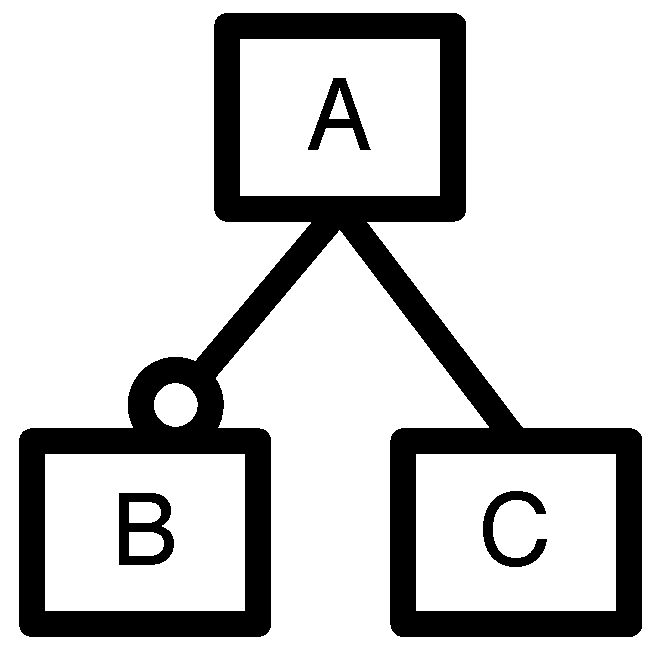
\includegraphics[width=15mm]{exemple-graphical-mutation-original}
		\label{fig:fmm:syntacticoriginal}
	}
	\subbottom[Mutant]{
		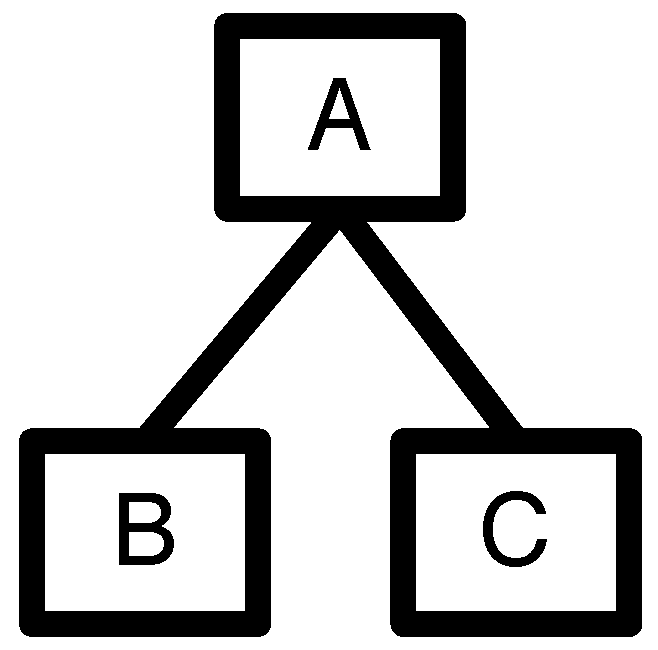
\includegraphics[width=15mm]{exemple-graphical-mutation-mutant}
		\label{fig:fmm:syntacticmutant}
	}
	\caption{Example of syntactic mutation of a feature model \cite{Arcaini2015a}}
	\label{fig:fmm:syntactic}
\end{figure}

Mutation operators working on the syntax of the feature model transform the graphical (or textual) representation of the feature model to produce a mutant. For instance, Arcaini \etal \cite{Arcaini2015a} define operators that will transform an alternative into a \textit{Or} or a \textit{And}, make an optional feature mandatory, change \textit{requires} constraint to \textit{exclude} constraint, \etc Figure \ref{fig:fmm:syntactic} presents an example of syntactic change in a small feature model: the optional constraint in Figure \ref{fig:fmm:syntacticoriginal} has been transformed to a mandatory feature in Figure \ref{fig:fmm:syntacticmutant}.

\paragraph{Semantic mutation:}
%-------------------------------

Semantic mutation works on the semantic of the feature model: a boolean expression over the features of the feature model \cite{Schobbens2007}. Application of those operators will first require a flattening of the feature model into a \gls{CNF} formula \cite{Henard2015b} and apply mutations on this formula. Henard \etal \cite{Henard2013b,Henard2014} use this strategy to select products to test in order to detect mutations of the feature model. The feature model is first transformed into a \gls{CNF} formula which is used an input for two mutation operators modifying on clause of the CNF formula. For instance, the feature model of Figure \ref{fig:fmm:syntacticoriginal} is transformed into the following CNF clause:
$$\fm = A \wedge (\neg B \vee A) \wedge (\neg C \vee A) \wedge (\neg A \vee C)$$
Which may then be mutated (using Henard \etal's \textit{second operator} \cite{Henard2013b}) to:
$$\fm_m = A \wedge \neg B \wedge A \wedge (\neg C \vee A) \wedge (\neg A \vee C)$$
%
Since the CNF formula represents the feature model, it is possible to show an equivalence between syntactic and semantic mutation operators. However, one application of a syntactic mutation operator may require several applications of semantic mutation operators (and \textit{vice versa}). For instance, the syntactic operator transforming an alternative to a \textit{And} will require several transformations on the CNF formula representing the feature model. 

\paragraph{Featured transition system mutation:}
%-------------------------------------------------

\begin{figure}
	\centering
	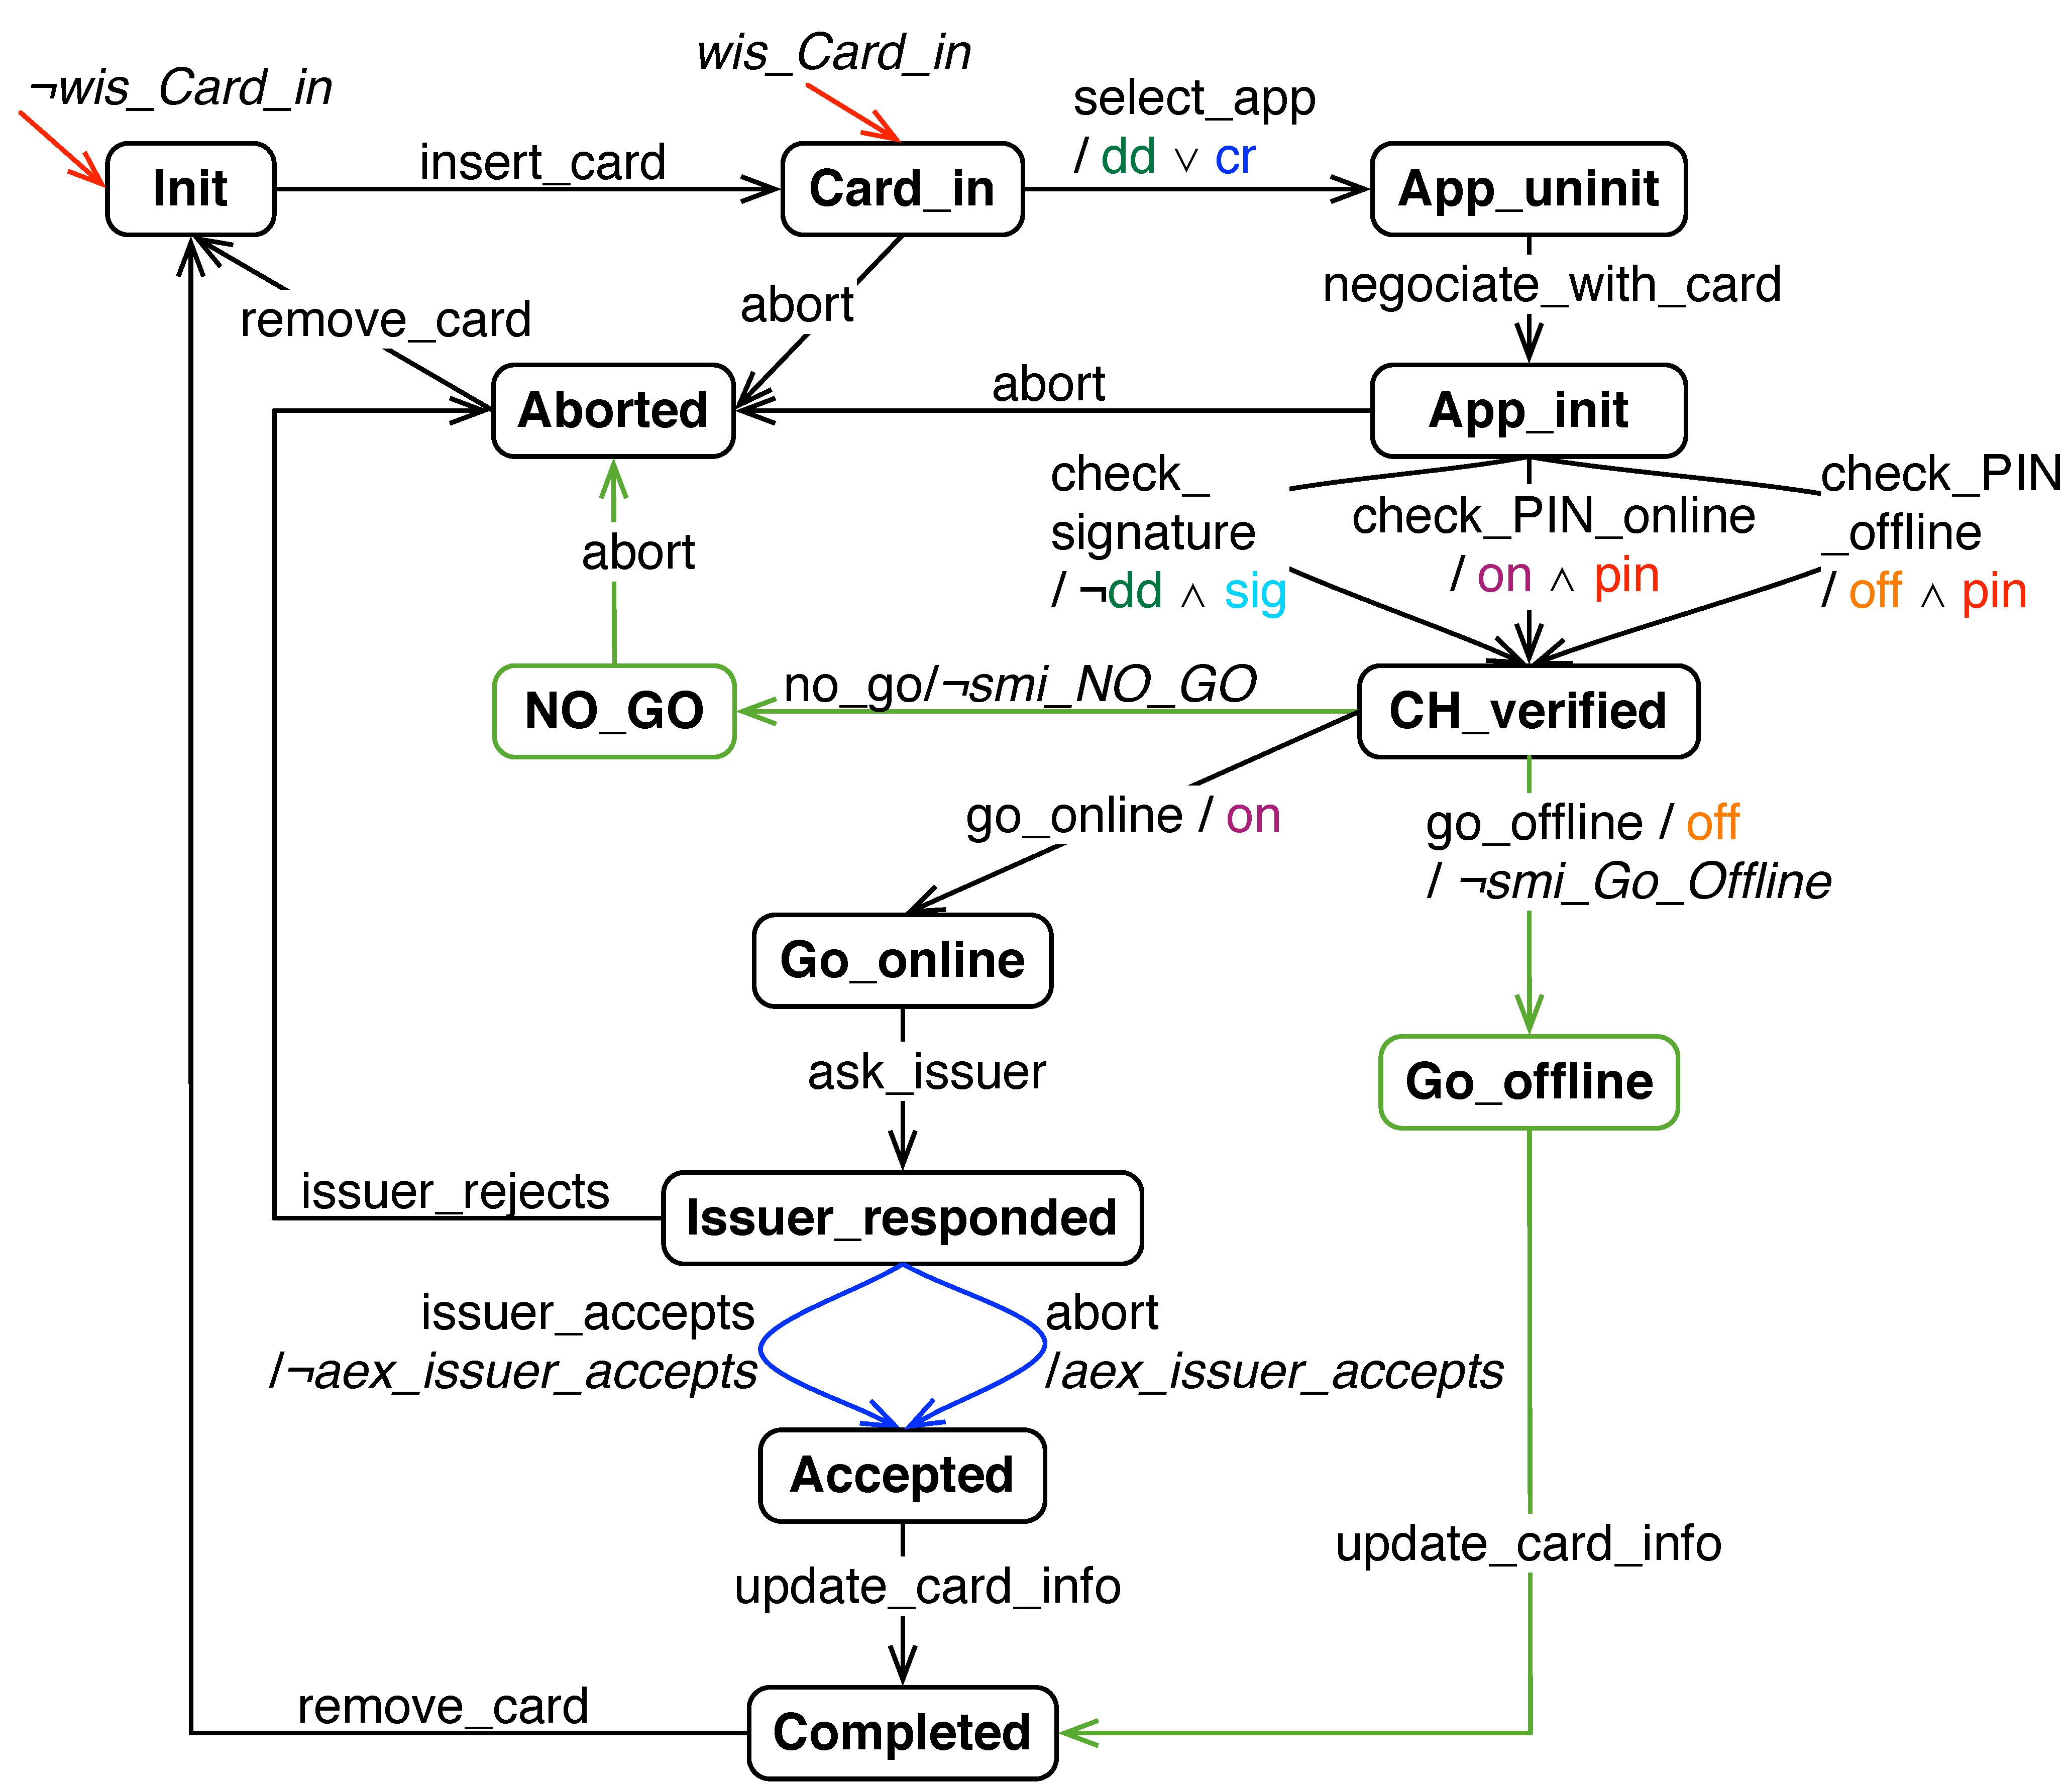
\includegraphics[width=95mm]{cpt-exemple-fts-fmm}
	\caption{Card payment terminal product line FFTS}
	\label{fig:fmm:ftsfmmexemple}
\end{figure}

\glspl{FTS} describe the behaviour of all the products of a product line. Mutate a FTS comes to modify the behaviour of a whole product line (or at least the products able to execute the modified part of the FTS). The mutation operators defined in Annex \ref{apdx:fmm:operators} may be used to produce mutants. In such case, the FMM has a FTS with two feature models and two $\gamma$ labelling functions. The first feature model $d_p$ and $\gamma_p$ function are used to represent all the products of the product line, and the second feature model $d_m$ and $\gamma_m$ function are used to represent all the mutants of the mutants family.
For instance, the result of the card payment terminal product line of Figures \ref{fig:cpterminalfts}, mutated using the state missing, action exchange, and wrong initial state operators, produces the FTS in Figure \ref{fig:fmm:ftsfmmexemple}. The FMM is composed of this FTS, the feature model of the product line (in Figure \ref{fig:cpterminalfm}), and the feature model of the mutants family (in Figure \ref{fig:fmm:cptmutantsfm}). 
As for feature model mutation, modifying the FTS using model transformations are \emph{syntactic mutations} and affects the product line as a whole. \Eg removing one transition using transition missing operator removes it for all the products of the product line.

\newcommand{\wFe}{\mathit{fe}}

One may want to mutate only the behaviour of a certain subset of products. In this case, the operators defined in Annex \ref{apdx:fmm:operators} have to be modified in order to consider only a given subset of products, represented as a feature expression $e$. For instance, if we mutate the following transition in an \emph{enumerative} way, with $e$ representing a subset of the products defined by the feature expression $\wFe$:
\begin{center}
\begin{tikzpicture}[>=stealth',shorten >=1pt,auto,node distance=4cm]
	\node[state] (s0) {$s_0$};
	\node[state] (s1) [right of=s0] {$s_1$};
	\path[->] (s0)  edge node {$\alpha_x / \wFe$} (s1);
\end{tikzpicture}
\end{center}
By applying the AEX operator to change action $\alpha_x$ to $\alpha_y$, but only for the subset of products designed by $e$, we have the mutant:
\begin{center}
\begin{tikzpicture}[>=stealth',shorten >=1pt,auto,node distance=4cm]
	\node[state] (s0) {$s_0$};
	\node[state] (s1) [right of=s0] {$s_1$};
	\path[->] (s0) edge node {$\alpha_y / \wFe \wedge e$} (s1)
	          (s0) edge [bend right=45] node [below] {$\alpha_x / \wFe \wedge \neg e$} (s1);
\end{tikzpicture}
\end{center}
Where the original transition is restricted to $ \wFe \wedge \neg e$ and the mutated transition is only activated for products respecting $\wFe \wedge e$ feature expression.
Using the \emph{\gls{FMM}} approach, we need to duplicate transitions to take the feature expression representing the mutant into account:
\begin{center}
\begin{tikzpicture}[>=stealth',shorten >=1pt,auto,node distance=4cm]
	\node[state] (s0) {$s_0$};
	\node[state] (s1) [right of=s0] {$s_1$};
	\path[->] (s0) edge node {$\alpha_x / \wFe / \neg aex$} (s1)
	          (s0) edge [bend left=45] node [above] {$\alpha_y / \wFe \wedge e / aex$} (s1)
	          (s0) edge [bend right=45] node [below] {$\alpha_x / \wFe \wedge \neg e / aex$} (s1);
\end{tikzpicture}
\end{center}
Modifying only a subset of the product line requires to take the \emph{semantic} of the FTS (\ie the FTS as a compact representation of all the products of the product line) into account.

\paragraph{Feature expression mutation:}
%----------------------------------------

\Glspl{feature expression} are boolean expressions over features. They are used to represent the set of products able to execute a given transition in a FTS: it \emph{maps} the variability defined in the feature model to the behavioural description of the product line. Feature expression mutation may be done using classical boolean mutation operators \cite{Mathur2008} in order to mutate this mapping.

\paragraph{Projection operator mutation:}
%-----------------------------------------

The projection operator is used to bind the variability in a given FTS by resolving the feature expressions for a given product: \ie an assignment of the feature variables, \textit{true} denoting a feature included in the product and \textit{false} a feature not included in the product. Mutate the projection operator introduces faults in the \emph{derivation process}, which results in a faulty specification of the product behaviour (\ie a wrong LTS). The mutation operators may include, for instance, switching feature assignment ($f$ becoming $\neg f$), considering all features to true or false, returning a constant value (all features expressions are evaluated to true of false), \etc

\paragraph{Wrap up:}
%-----------------------------------------

In this section, we present possible solutions and research directions to apply a model-based product line mutation analysis. Mutation may be done using different \emph{artefacts} as inputs of the mutation operators and works at different levels of abstraction. We distinct mutation performed at \emph{syntactic} level from mutation at \emph{semantic} level. 
%
Both syntactic and semantic mutations of the feature model changes the set of valid products of the SPL. Existing approaches may be included in VIBeS. Those kinds of mutations may be detected by a test case, if one of the transitions fired by this test case on the original system may not be fired any more on the mutant. Concretely, the feature expression of this transition has to violate the constraints of the mutant feature model. 
%
FTS mutation for only a subset of the product line requires to modify the existing set of mutation operators (defined in Annex \ref{apdx:fmm:operators}). We believe that those mutations are more subtle as they allow to modify only a limited subset of the products, corresponding intuitively to undesired feature interactions (at the model level) preventing this subset of products to behave as expected.
%
Other kinds of mutation includes mutation of the feature expressions in the FTS (using classical boolean mutation operators) and mutation of the projection operator (using new operators).

\paragraph{Future work:}
%-----------------------------------------

In our future work, we will refine the vision sketched here and enhance VIBeS's mutation analysis by following the aforementioned directions.
We will also further investigate scalability issues regarding mutation analysis for any order mutants. This implies the optimisation of the boolean formulas or approximate computation heuristics. To address the equivalent mutant problem in a family-based fashion, we intent to investigate usage of automata language equivalence (or other equivalence approaches) for FTSs. For now, FMMs are used only to represent behavioural mutations. We intend to extend this set of mutation operators to mutate variability information of the input FTS and feature model. Finally, scalability of mutation analysis for large \glspl{SPL} has to be evaluated in the long run.


%%%%%%%%%%%%%%%%%%%%%%%%%%
\section{Final remarks}
%%%%%%%%%%%%%%%%%%%%%%%%%%

This thesis is dedicated to \gls{SPL} testing but we believe that the contributions may be extended to other kinds of systems. \glspl{SPL} are variability intensive systems that have been developed in a structured process, divided into domain engineering and application engineering \cite{Pohl2005}. But variability is not limited to product lines. As suggested by the name of our implementation \acrfull{VIBeS} and the Web application case studies used in this thesis, our work may be used to test other sorts of systems: plugin-based system like WordPress for instance. 

Relevant test suites and products selection becomes even more important considering the way software is developed nowadays. For instance, Agile methods, continuous integration and delivery, and fast releasing requires to execute test cases using a limited testing budget (usually overnight), making test cases selection critical to ensure a required quality level. This also raises further research directions: for now, VIBeS' inputs are a FTS and its feature model. Since FTS is an abstract formalism, it allows to be expressed using other modelling languages like fPromela \cite{Classen2013b}, dedicated to FTS model checking. We believe that using lightweight modelling languages dedicated to testing (like Gherkin \cite{cucumber}) with variability information may foster the adoption of SPL testing techniques and help the community to master the variability more and more present in software systems. 

With the emergence of the so-called \textit{DevOps}, development and system operation teams inside an organisation are aligned and collaborate intensively to ensure rapid, frequent, and reliable software building, testing, and delivery. This includes a sharing of information between development environment and operating environment. In such case, the input model may even be enhanced (automatically or not) with other kinds of information automatically inferred from the running systems, the versioning engine, or the continuous integration server. This allows to tailor and refine the test case selection even further. It would allow to include variability intensive systems in a continuous test cycle, where test cases are selected and executed based on inputs from different sources contributing to a continuous quality improvement cycle.

